\documentclass[answers]{exam}
\usepackage{marvosym}

%...TikZ & PGF
\usepackage{pgfplots}
\pgfplotsset{compat=1.11}
\tikzset{>=latex}
\usetikzlibrary{calc,math}
\usepackage{tikzsymbols}
\usepgfplotslibrary{fillbetween}
\usetikzlibrary{decorations.markings} 
\usetikzlibrary{arrows.meta} %...APP2 for arrows as objects and images
\usetikzlibrary{backgrounds} %...For shading portions of graphs
\usetikzlibrary{patterns} %...Unit 5 Problems
\usetikzlibrary{shapes.geometric} %...For drawing cylinders in Unit 2
\tikzset{
    mark position/.style args={#1(#2)}{
        postaction={
            decorate,
            decoration={
                markings,
                mark=at position #1 with \coordinate (#2);
            }
        }
    }
} %...See https://tex.stackexchange.com/questions/43960/define-node-at-relative-coordinates-of-draw-plot

\tikzset{
    declare function = {trajectoryequation10(\x,\vi,\thetai)= tan(\thetai)*\x - 10*\x^2/(2*(\vi*cos(\thetai))^2);},
    declare function = {trajectoryequation(\x,\vi,\thetai)= tan(\thetai)*\x - 9.8*\x^2/(2*(\vi*cos(\thetai))^2);},
    declare function = {patheq(\x,\yi,\vi,\thetai)= \yi + tan(\thetai)*\x - 9.8*\x^2/(2*(\vi*cos(\thetai))^2);},
    declare function = {patheqten(\x,\yi,\vi,\thetai)= \yi + tan(\thetai)*\x - 10*\x^2/(2*(\vi*cos(\thetai))^2);} %like patheq but with gravity = 10
}

%...siunitx
\usepackage{siunitx}
\DeclareSIUnit{\nothing}{\relax}
\def\mymu{\SI{}{\micro\nothing} }
\DeclareSIUnit\mmHg{mmHg}
\DeclareSIUnit{\mile}{mi}
%...NOTE: "The product symbol between the number and unit is set using the quantity-product option."

%...Other
\usepackage{amsthm}
\usepackage{amsmath}
\usepackage{amssymb}
\usepackage{cancel}
\usepackage{subcaption}
\usepackage{dashrule}
\usepackage{enumitem}
\usepackage{fontawesome}
\usepackage{multicol}
\usepackage{glossaries}
%\numberwithin{equation}{section}
\numberwithin{figure}{section}
\usepackage{float}
\usepackage{twemojis} %...twitter emojis
\usepackage{utfsym}
\newcommand{\R}{\mathbb{R}} %...real number symbol
\usepackage{graphicx}
\graphicspath{ {../Figures/} }
\usepackage{hyperref}
\hypersetup{colorlinks=true,
    linkcolor=blue,
    filecolor=magenta,
    urlcolor=cyan,}
\urlstyle{same}
\newcommand{\hdashline}{{\hdashrule{\textwidth}{0.5pt}{0.8mm}}}
\newcommand{\hgraydashline}{{\color{lightgray} \hdashrule{0.99\textwidth}{1pt}{0.8mm}}}

%...Miscellaneous user-defined symbols
\newcommand{\fnet}{F_{\text{net}}} %...For net force
\newcommand{\bvec}[1]{\vec{\mathbf{#1}}} %...bold vector
\newcommand{\bhat}[1]{\,\hat{\mathbf{#1}}} %...bold hat vector
\newcommand{\que}{\mathord{?}}  %...Question mark symbol in equation env
%...Define thick horizontal rule for examples:
\newcommand{\hhrule}{\hrule\hrule}
\let\oldtexttt\texttt% Store \texttt
\renewcommand{\texttt}[2][black]{\textcolor{#1}{\ttfamily #2}}% 

%...For use in the exam document class
\newif\ifprintmetasolutions


%...Decreases space above and below align and gather enironment
\makeatletter
\g@addto@macro\normalsize{%
  \setlength\abovedisplayskip{-3pt}
  \setlength\belowdisplayskip{6pt} 
}
\makeatother






\begin{document}

\begin{questions}
\question
Consider the following motion graph.

\begin{center}
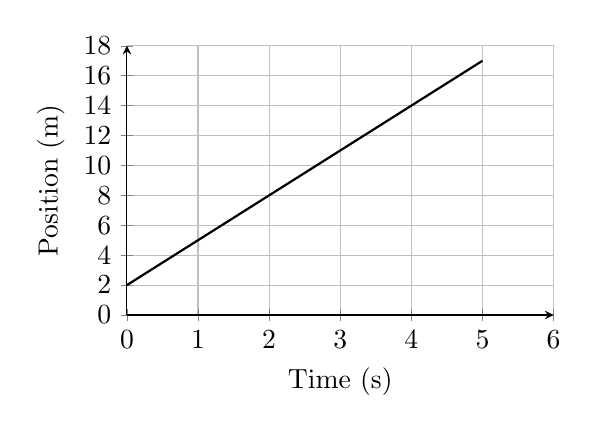
\begin{tikzpicture}
    \begin{axis}[height=5cm,
        width=7cm,
        axis lines=left,
        ylabel={Position (m)},
        xlabel={Time (s)},
        ymin=0,ymax=18,
        xmin=0,xmax=6,
        ytick={0,2,...,18},
        xtick={0,1,...,6},
        grid=both,
    ]
        \addplot[thick,domain=0:5] {3*x+2};
    \end{axis}
\end{tikzpicture}
\end{center}

\begin{parts}
\part 
Which is the independent variable?

\begin{solution}
    Time
\end{solution}

\part 
Which is the dependent variable?

\begin{solution}
    Position
\end{solution}

\part
Where was the object at 4 seconds?

\begin{solution}
    \SI{14}{m}
\end{solution}

\part
Find the slope of the graph. Show all your work.

\begin{solution}
\begin{center}
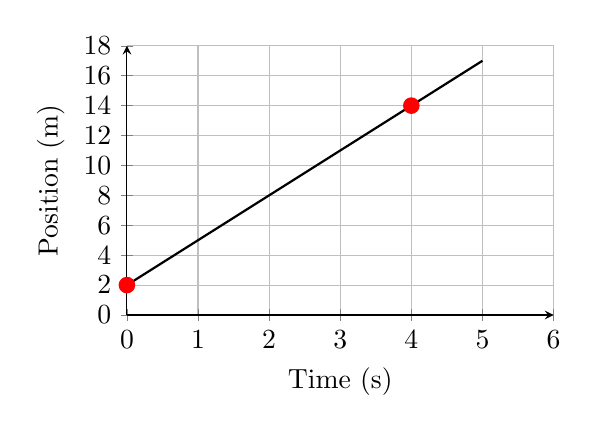
\begin{tikzpicture}
    \begin{axis}[height=5cm,
        width=7cm,
        axis lines=left,
        ylabel={Position (m)},
        xlabel={Time (s)},
        ymin=0,ymax=18,
        xmin=0,xmax=6,
        ytick={0,2,...,18},
        xtick={0,1,...,6},
        grid=both,
        clip=false,
    ]
        \addplot[thick,domain=0:5] {3*x+2};
        \fill[red] (0,2) circle (3pt);
        \fill[red] (4,14) circle (3pt);
    \end{axis}
\end{tikzpicture}
\end{center}

Using the two coordinates shown above, the slope is rise over run:

\begin{equation*}
    \text{slope} = \frac{\SI{14}{m} - \SI{2}{m}}{\SI{4}{s} - \SI{0}{s}} = \boxed{\SI{3}{m/s}}
\end{equation*}
\end{solution}


\part 
What physical quantity does the slope represent?


\end{parts}

\end{questions}
\end{document}